\documentclass[]{elsarticle} %review=doublespace preprint=single 5p=2 column
%%% Begin My package additions %%%%%%%%%%%%%%%%%%%
\usepackage[hyphens]{url}

  \journal{Building and Environment} % Sets Journal name


\usepackage{lineno} % add
\providecommand{\tightlist}{%
  \setlength{\itemsep}{0pt}\setlength{\parskip}{0pt}}

\usepackage{graphicx}
\usepackage{booktabs} % book-quality tables
%%%%%%%%%%%%%%%% end my additions to header

\usepackage[T1]{fontenc}
\usepackage{lmodern}
\usepackage{amssymb,amsmath}
\usepackage{ifxetex,ifluatex}
\usepackage{fixltx2e} % provides \textsubscript
% use upquote if available, for straight quotes in verbatim environments
\IfFileExists{upquote.sty}{\usepackage{upquote}}{}
\ifnum 0\ifxetex 1\fi\ifluatex 1\fi=0 % if pdftex
  \usepackage[utf8]{inputenc}
\else % if luatex or xelatex
  \usepackage{fontspec}
  \ifxetex
    \usepackage{xltxtra,xunicode}
  \fi
  \defaultfontfeatures{Mapping=tex-text,Scale=MatchLowercase}
  \newcommand{\euro}{€}
\fi
% use microtype if available
\IfFileExists{microtype.sty}{\usepackage{microtype}}{}
\usepackage[left=2.5cm,right=2.5cm,top=2.5cm,bottom=2.5cm]{geometry}
\bibliographystyle{elsarticle-harv}
\usepackage{color}
\usepackage{fancyvrb}
\newcommand{\VerbBar}{|}
\newcommand{\VERB}{\Verb[commandchars=\\\{\}]}
\DefineVerbatimEnvironment{Highlighting}{Verbatim}{commandchars=\\\{\}}
% Add ',fontsize=\small' for more characters per line
\usepackage{framed}
\definecolor{shadecolor}{RGB}{248,248,248}
\newenvironment{Shaded}{\begin{snugshade}}{\end{snugshade}}
\newcommand{\AlertTok}[1]{\textcolor[rgb]{0.94,0.16,0.16}{#1}}
\newcommand{\AnnotationTok}[1]{\textcolor[rgb]{0.56,0.35,0.01}{\textbf{\textit{#1}}}}
\newcommand{\AttributeTok}[1]{\textcolor[rgb]{0.77,0.63,0.00}{#1}}
\newcommand{\BaseNTok}[1]{\textcolor[rgb]{0.00,0.00,0.81}{#1}}
\newcommand{\BuiltInTok}[1]{#1}
\newcommand{\CharTok}[1]{\textcolor[rgb]{0.31,0.60,0.02}{#1}}
\newcommand{\CommentTok}[1]{\textcolor[rgb]{0.56,0.35,0.01}{\textit{#1}}}
\newcommand{\CommentVarTok}[1]{\textcolor[rgb]{0.56,0.35,0.01}{\textbf{\textit{#1}}}}
\newcommand{\ConstantTok}[1]{\textcolor[rgb]{0.00,0.00,0.00}{#1}}
\newcommand{\ControlFlowTok}[1]{\textcolor[rgb]{0.13,0.29,0.53}{\textbf{#1}}}
\newcommand{\DataTypeTok}[1]{\textcolor[rgb]{0.13,0.29,0.53}{#1}}
\newcommand{\DecValTok}[1]{\textcolor[rgb]{0.00,0.00,0.81}{#1}}
\newcommand{\DocumentationTok}[1]{\textcolor[rgb]{0.56,0.35,0.01}{\textbf{\textit{#1}}}}
\newcommand{\ErrorTok}[1]{\textcolor[rgb]{0.64,0.00,0.00}{\textbf{#1}}}
\newcommand{\ExtensionTok}[1]{#1}
\newcommand{\FloatTok}[1]{\textcolor[rgb]{0.00,0.00,0.81}{#1}}
\newcommand{\FunctionTok}[1]{\textcolor[rgb]{0.00,0.00,0.00}{#1}}
\newcommand{\ImportTok}[1]{#1}
\newcommand{\InformationTok}[1]{\textcolor[rgb]{0.56,0.35,0.01}{\textbf{\textit{#1}}}}
\newcommand{\KeywordTok}[1]{\textcolor[rgb]{0.13,0.29,0.53}{\textbf{#1}}}
\newcommand{\NormalTok}[1]{#1}
\newcommand{\OperatorTok}[1]{\textcolor[rgb]{0.81,0.36,0.00}{\textbf{#1}}}
\newcommand{\OtherTok}[1]{\textcolor[rgb]{0.56,0.35,0.01}{#1}}
\newcommand{\PreprocessorTok}[1]{\textcolor[rgb]{0.56,0.35,0.01}{\textit{#1}}}
\newcommand{\RegionMarkerTok}[1]{#1}
\newcommand{\SpecialCharTok}[1]{\textcolor[rgb]{0.00,0.00,0.00}{#1}}
\newcommand{\SpecialStringTok}[1]{\textcolor[rgb]{0.31,0.60,0.02}{#1}}
\newcommand{\StringTok}[1]{\textcolor[rgb]{0.31,0.60,0.02}{#1}}
\newcommand{\VariableTok}[1]{\textcolor[rgb]{0.00,0.00,0.00}{#1}}
\newcommand{\VerbatimStringTok}[1]{\textcolor[rgb]{0.31,0.60,0.02}{#1}}
\newcommand{\WarningTok}[1]{\textcolor[rgb]{0.56,0.35,0.01}{\textbf{\textit{#1}}}}
\usepackage{longtable}
\ifxetex
  \usepackage[setpagesize=false, % page size defined by xetex
              unicode=false, % unicode breaks when used with xetex
              xetex]{hyperref}
\else
  \usepackage[unicode=true]{hyperref}
\fi
\hypersetup{breaklinks=true,
            bookmarks=true,
            pdfauthor={},
            pdftitle={A big change!},
            colorlinks=true,
            urlcolor=blue,
            linkcolor=blue,
            pdfborder={0 0 0}}
\urlstyle{same}  % don't use monospace font for urls

\setcounter{secnumdepth}{5}
% Pandoc toggle for numbering sections (defaults to be off)


% Pandoc header
\usepackage{setspace}
\doublespacing
\usepackage[font={small}]{caption}
\usepackage{amsmath}
\usepackage{booktabs}
\usepackage{caption}
\usepackage{longtable}



\begin{document}
\begin{frontmatter}

  \title{A big change!}
    \author[CBE]{Paul Raftery\corref{Corresponding Author}}
   \ead{p.raftery@berkeley.edu} 
    \author[CBE]{Dana Miller}
  
    \author[Organization2]{Next contributor}
  
      \address[CBE]{Center for the Built Environment, UC Berkeley, 390 Wurster Hall, Berkeley, CA, 94720, USA}
    \address[Organisation2]{Another organization, and their address}
    
  \begin{abstract}
  Enter the text for your abstract here. All data and analysis code in this template is publicly available at \url{https://github.com/CenterForTheBuiltEnvironment/rmd-example} and can be freely adapted and reused. Suggestions or pull requests to improve this template or create additional templates are welcome.
  \end{abstract}
  
 \end{frontmatter}

Keywords:\\
Keyword 1; Keyword 2; Keyword 3; Keyword 4; Keyword 5; Keyword 6 (max)

\pagebreak

\textbf{Highlights:}

\begin{itemize}
\tightlist
\item
  Add your 3 -5 highlights
\item
  As bulletpoints here
\item
  Making sure each is less than 85 characters in length
\end{itemize}

\textbf{Graphical Abstract}


\includegraphics[width=4.44in]{/home/trc/rmd-example/Paper/SupplementaryMaterial/Images/Latex_logo}

\pagebreak

\hypertarget{introduction}{%
\section{Introduction}\label{introduction}}

The purpose of this (very much work-in-progress) document is to provide a complete R markdown template for an Elsevier journal submission (based on the \href{https://github.com/rstudio/rticles}{rticles} repository Allaire et al. (\protect\hyperlink{ref-rticles}{2017})), along with useful examples and packages to improve usability for folks who are just starting out with this workflow. The eventual intent is to capture minimal examples of the common things that authors need to do when writing papers in R markdown; provide examples of useful packages, workflows, and tools; and provide solutions to common issues that folks encounter.

You may wish to have short sub-sections for:

\begin{itemize}
\tightlist
\item
  Terminology
\item
  Objectives
\end{itemize}

\hypertarget{methods-this-is-a-level-1-heading}{%
\section{Methods (this is a `level 1 heading')}\label{methods-this-is-a-level-1-heading}}

\hypertarget{markdown-this-is-a-level-2-heading}{%
\subsection{Markdown (this is a `level 2 heading')}\label{markdown-this-is-a-level-2-heading}}

This RMarkdown document is a special type of interactive document that can contain both code chunks (in R, python, or other languages), and text written in a format called Markdown. Here are some examples of how to format text with Markdown, and a \href{https://www.rstudio.com/wp-content/uploads/2015/03/rmarkdown-reference.pdf}{link} to an RMarkdown guide.

\hypertarget{level-3-heading}{%
\subsubsection{Level 3 heading}\label{level-3-heading}}

Here's how to \textbf{bold} or \emph{italicize} a piece of text. This is how you do a bullet point list:

\begin{itemize}
\tightlist
\item
  First bullet
\item
  Second bullet

  \begin{itemize}
  \tightlist
  \item
    A sub-bullet
  \item
    Another sub-bullet
  \end{itemize}
\end{itemize}

Or an ordered option:

\begin{enumerate}
\def\labelenumi{\arabic{enumi}.}
\tightlist
\item
  Item 1
\item
  Item 2

  \begin{itemize}
  \tightlist
  \item
    Item 2a
  \item
    Item 2b
  \end{itemize}
\end{enumerate}

\hypertarget{tables}{%
\subsection{Tables}\label{tables}}

Here is an example of a table created from the .csv file in the \texttt{SupplementaryMaterial/Data}folder using the \texttt{gt} package from RStudio. You can read more about \texttt{gt} \href{https://github.com/rstudio/gt}{here}, and there's helpful examples to further customize tables (eg with color, footnotes, significant figures, re-labeling columns, and more) \href{https://github.com/allisonhorst/gt-awesome-tables}{here}.

\captionsetup[table]{labelformat=empty,skip=1pt}
\begin{longtable}{lrrc}
\caption*{
\large Example irises\\ 
\small Data on five randomly selected irises\\ 
} \\ 
\toprule
iris\_class & sepal\_length & petal\_length & petal\_length\_level \\ 
\midrule
Iris-setosa & 5.3 & 1.5 & Low \\ 
Iris-versicolor & 5.6 & 3.6 & Medium \\ 
Iris-versicolor & 6.1 & 4.7 & High \\ 
Iris-virginica & 6.7 & 5.2 & High \\ 
Iris-virginica & 5.6 & 4.9 & High \\ 
\bottomrule
\end{longtable}

\hypertarget{spellcheck}{%
\subsection{Spellcheck}\label{spellcheck}}

If you are using RStudio, press F7 or go to \texttt{Edit} --\textgreater{} \texttt{Check\ spelling} in the menu.

\hypertarget{cross-referencing}{%
\subsection{Cross-referencing}\label{cross-referencing}}

This is how you refer to a figure in your text: Figure \ref{fig:correlation}. Simply reference the title of the code chunk, and ensure that the code chunk includes a figure caption.

\begin{figure}[h]
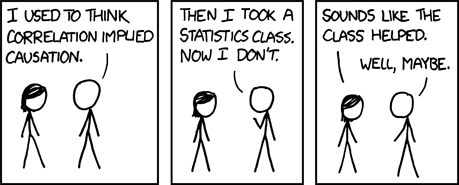
\includegraphics[width=0.92in]{/home/trc/rmd-example/Paper/SupplementaryMaterial/Images/correlation} \caption{Correlation. Source: XKCD, xkcd.com/552}\label{fig:correlation}
\end{figure}

\hypertarget{calculations-in-text}{%
\subsection{Calculations in text}\label{calculations-in-text}}

The holy grail of markdown - doing all of your calculations in the same file so you never need to worry about updating them after someone\footnote{Often I'm the someone, sorry CBE grad students. Also, look, it's an example of a footnote!} asks you to make changes\ldots{}. again! It's as easy as pi: 3.14. Incidentally,you can selectively override the `global' options set at the beginning, to say for example, show more decimals: 3.1416.

This is an example of outputing the result of a calculation that you perform within a code chunk in the document somewhere prior to the location where you first refer to it: 36.

\hypertarget{citations}{%
\subsection{Citations}\label{citations}}

\hypertarget{citing-literature}{%
\subsubsection{Citing literature}\label{citing-literature}}

Citing other literature is remarkably easy, just like this Coakley et al. (\protect\hyperlink{ref-coakleyReviewMethodsMatch2014}{2014}). This citation key references the tag associated with an entry in Bibliography.bib (a BibTex file). I've found it easiest to use Zotero to manage my library of references and to generate the BibTex file, though any software that creates a valid BibTex file should work fine. Zotero allows you to create a `Collection' (or folder) that gathers together all of the references used for a particular document. When combined with with the Better BibTex plugin, that collection can be exported to a BibTex file that is continually updated as you add or edit references in that Collection. Better BibTex also puts the citation key - the text after the `@' symbol in the .Rmd file - on the upper right of each entry, which is convenient for adding citations.

There's not much else involved in citing, as the references list gets built and formatted automatically based on the selected style. The only other issue I've had to look around to solve was figuring out how to combine multiple citations, which is easy when you know how. (Coakley et al., \protect\hyperlink{ref-coakleyReviewMethodsMatch2014}{2014}; Zhai et al., \protect\hyperlink{ref-zhaiHumanComfortPerceived2015a}{2015})

\textbf{Step-by-step instructions for creating a new Zotero collection and adding a citation}
1. Install BetterBibtex with the instructions \href{https://retorque.re/zotero-better-bibtex/}{here}.

\begin{enumerate}
\def\labelenumi{\arabic{enumi}.}
\setcounter{enumi}{1}
\item
  First, create a new Zotero collection for this paper in your own Zotero library. You can add existing references by dragging and dropping them into the folder for this collection, or add new references from the web with this collection highlighted.
\item
  In the far left Zotero pane, right-click on the folder for this collection, select ``Export Collection'', and selection ``Better BibTeX'' and the format, and tick the ``Keep updated'' box (this will automatically update the stored .bib file when you add new items to this collection). Save this .bib file in a location together with the document you are working on (in this repository, it's under \texttt{/Paper})

  \begin{itemize}
  \tightlist
  \item
    Note - the dynamic updating \emph{only} works if you export the whole collection to one .bib file, so clicking on the items in the collection and exporting them individually or together will not work
  \end{itemize}
\item
  To add a citation in the text, first make sure that the item is saved in the Zotero collection that is linked to the automatically-updating .bib file for your document. Then click on that item in Zotero and copy the citation key in the right-hand pane (eg \emph{schiavonThermalComfortPerceived2017})
\item
  In your document, paste the citation key preceded by an @ sign, like this: \texttt{@schiavonThermalComfortPerceived2017} in the text where you want the citation to appear. If you want it wrapped in parentheses, do this \texttt{{[}@schiavonThermalComfortPerceived2017{]}}
\end{enumerate}

\hypertarget{citing-software}{%
\subsubsection{Citing software}\label{citing-software}}

It is also good practice to include citations for the software used in your analysis. After all, the software is also one of the tools you used to carry out your research. It is important to attribute which software and which versions you used you used so other people can better understand your methods. There have been cases where running the same analysis code with different versions of the same software produces different results! In addition, citing software helps to provide credit for the creators and maintainers of the software and demonstrate that people are using it, which is especially important for open-source tools supported through public research funding. Just like software often includes a \texttt{LICENSE} file, a good practice is for citation instructions to be included in a \texttt{CITATION} file associated with the project. Many software packages have accompanying publications that can be cited, and if they don't there is usually a project website or code repository.

\textbf{Instructions for adding software citations with \texttt{grateful} and Zotero}

\begin{Shaded}
\begin{Highlighting}[]
\CommentTok{# Example of generating BibTex file for the packages listed below}
\CommentTok{# Note the output location is specified }
\CommentTok{# Note tidyverse is not included in the list below because it's a large package to install on Binder, if you are running this on your own computer I recommend including it if you want to cite it}
\NormalTok{pkgs <-}\StringTok{ }\KeywordTok{c}\NormalTok{(}\StringTok{"here"}\NormalTok{, }\StringTok{"knitr"}\NormalTok{, }\StringTok{"ggpmisc"}\NormalTok{, }\StringTok{"gt"}\NormalTok{, }\StringTok{"grateful"}\NormalTok{, }\StringTok{"base"}\NormalTok{, }\StringTok{"rticles"}\NormalTok{, }\StringTok{"bookdown"}\NormalTok{, }
          \StringTok{"rmarkdown"}\NormalTok{)}
\NormalTok{cites <-}\StringTok{ }\NormalTok{grateful}\OperatorTok{::}\KeywordTok{get_citations}\NormalTok{(pkgs, }\DataTypeTok{filename =} \StringTok{"pkg-refs.bib"}\NormalTok{,}
                    \DataTypeTok{out.dir =}  \KeywordTok{here}\NormalTok{(}\StringTok{"/Paper/SupplementaryMaterial/Software_citations"}\NormalTok{) )}
\end{Highlighting}
\end{Shaded}

\begin{enumerate}
\def\labelenumi{\arabic{enumi}.}
\setcounter{enumi}{4}
\item
  To add software citations, you can use the \texttt{greatful} package's \texttt{get\_citations} function to generate the BibTeX-formatted citation for each package. Note that all of the packages have to be loaded into your working session, and listed before calling \texttt{get\_citations} for this to work.
\item
  Next, open the \texttt{pkg-refs.bib} file generated by \texttt{greatful} in a text editor like Notepad, highlight and copy the text, and then in Zotero with the collection for this project highlighted, click \texttt{File} --\textgreater{} \texttt{Import\ from\ clipboard}. Now all the software references have been added to the .bib file that will continue to be updated for this project!
\item
  Cite the software somewhere in your methods section. Here's an example:
\end{enumerate}

\begin{quote}
This paper used the free and open source R statistical computing language (R Core Team, \protect\hyperlink{ref-base}{2018}) with \texttt{tidyverse} (Wickham, \protect\hyperlink{ref-tidyverse}{2017}) software for all analysis, with the additional software packages \texttt{ggpmisc} (Aphalo, \protect\hyperlink{ref-ggpmisc}{2016}) for graphics, \texttt{gt} (Iannone et al., \protect\hyperlink{ref-gt}{2019})for tables, \texttt{here} (Müller, \protect\hyperlink{ref-here}{2017}) for file path management, \texttt{grateful} (Rodriguez-Sanchez, \protect\hyperlink{ref-grateful}{2018}) for software citation, \texttt{rmarkdown} (Allaire et al., \protect\hyperlink{ref-rmarkdown}{2018}) for interactive notebooks, and \texttt{knitr} (Xie, \protect\hyperlink{ref-knitr}{2018}), \texttt{rticles} (Allaire et al., \protect\hyperlink{ref-rticles}{2017}), and \texttt{bookdown} (Xie, \protect\hyperlink{ref-bookdown}{2016}) to create a journal-formatted PDF and other markdown and html files.
\end{quote}

\hypertarget{equations-and-math}{%
\subsection{Equations and math}\label{equations-and-math}}

Here's a basic example inline \(example_{subscript} = \frac{D}{R}\), or you display it on a whole line if needed. Google latex math cheat sheets for more information.

\[\sum_{i=1}^{n}{x_i^2}\]

Here is another equation:

\[ CD_{rated} = \frac{4*Q}{\pi*D^2} = 2.0~m/s\]

\hypertarget{other-packages}{%
\subsection{Other packages}\label{other-packages}}

There are lots of packages that are useful for markdown docs and customizing plots. We encourage you to search for these whenever you encounter a new thing you need to do and to propose an addition to this repository accordingly. Some examples to start: \texttt{ggExtra}, \texttt{gridExtra}, \texttt{RColorBrewer}, \texttt{ggrepel}\ldots{}

\hypertarget{writing-style}{%
\subsection{Writing style}\label{writing-style}}

This is a little off topic for an Rmd example but a convenient place to remind our grad students about writing style. In almost all cases, active voice is better than passive voice. Several psychological studies show that the active voice is more easily understood by readers, and that information is more accurately reported by authors when writing in active voice. For example, research Klenbort \& Anisfeld (\protect\hyperlink{ref-klenbortMarkednessPerspectiveInterpretation1974}{1974}) has shown that the ``active {[}voice{]} offers a neutral structure for conveying information''. Authorship guides for highly regarded journals often indicate a preference for the active voice instead of passive:

\begin{itemize}
\tightlist
\item
  Nature: ``Nature journals like authors to write in the active voice (`we performed the experiment\ldots{}') as experience has shown that readers find concepts and results to be conveyed more clearly if written directly.''(\emph{Nature - How to Write a Paper}, n.d.)
\item
  Science: ``Use active voice when suitable, particularly when necessary for correct syntax (e.g., `To address this possibility, we constructed a lZap library \ldots{},' not `To address this possibility, a lZap library was constructed\ldots{}').'' Ruben et al. (\protect\hyperlink{ref-rubenHowWriteScientist2012}{2012})
\end{itemize}

And, on top of all that, you also end up with less text if you write in active voice, saving space for useful information and making it easier for your readers to understand.

\hypertarget{a-fun-way-to-spot-passive-voice}{%
\subsubsection{A fun way to spot passive voice:}\label{a-fun-way-to-spot-passive-voice}}

If you can add the words `by zombies' (``A Scary-Easy Way to Help You Find Passive Voice!'' \protect\hyperlink{ref-ScaryeasyWayHelp2014}{2014}) to the end of the sentence and the sentence still makes logical sense, then the sentence is in passive voice. You can also switch on the grammar settings in Microsoft Word's spelling and grammar checker and it will show up that way.

How to fix it?

Change:

``These measurements are not quantitatively reported in the paper'' (\ldots{} by zombies)

To

``The paper does not quantitatively report these measurements''

Or even better, it's really the authors doing the reporting as the paper is an inanimate object\ldots{}

``We do not quantitatively report these measurements''.

Change:

``Six different table and partition configurations were tested'' (\ldots{} by zombies)

To

``We tested six different table and partition configurations.''

\hypertarget{results}{%
\section{Results}\label{results}}

\hypertarget{scatter-plot-example}{%
\subsection{Scatter plot example}\label{scatter-plot-example}}

Figure \ref{fig:irises} shows petal widths by iris type.

\begin{figure}[h]

{\centering 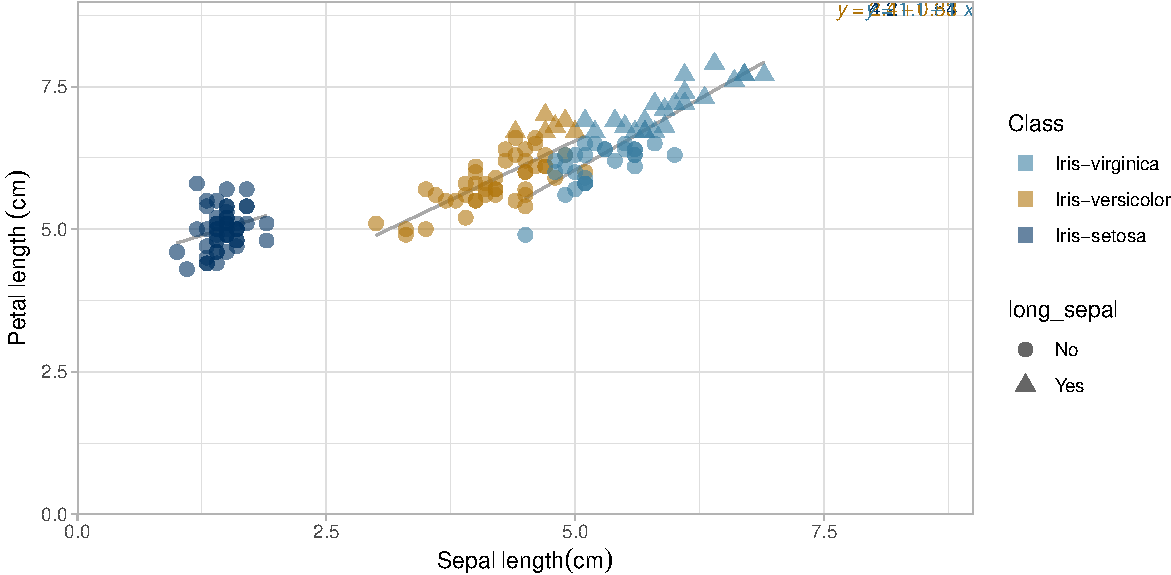
\includegraphics{Manuscript_files/figure-latex/irises-1} 

}

\caption{Petal and sepal lengths from iris dataset}\label{fig:irises}
\end{figure}

\hypertarget{violin-plot-example}{%
\subsection{Violin plot example}\label{violin-plot-example}}

Figure \ref{fig:petalwidths} shows petal widths by iris type.

\begin{figure}[h]

{\centering 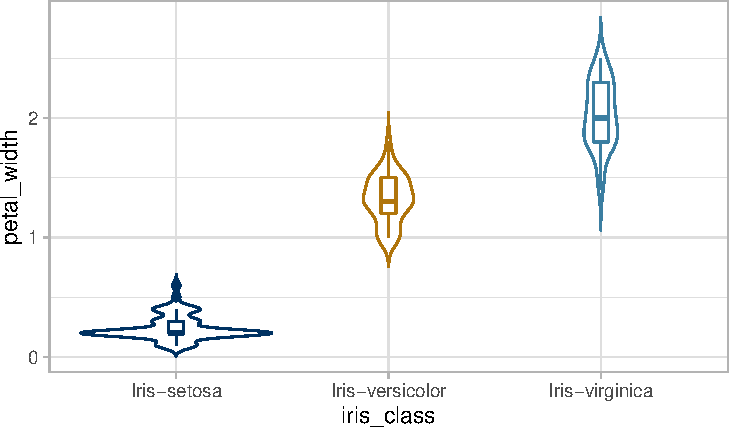
\includegraphics{Manuscript_files/figure-latex/petalwidths-1} 

}

\caption{Iris petal widths by species}\label{fig:petalwidths}
\end{figure}

\hypertarget{discussion}{%
\section{Discussion}\label{discussion}}

\hypertarget{limitations}{%
\section{Limitations}\label{limitations}}

It is important to include a discussion of limitations in any paper. Some limitations of this template include:

\begin{itemize}
\tightlist
\item
  Whether or not figures are included inline with text appears to depend of the version of LaTeX the document is compiled with. Compiling on a computer where TinyTeX is installed (eg in the Binder associated with the repository for this project on GitHub) will render the figures inline, whereas compiling the same document on a Windows computer with MikTeX installed does not
\item
  Does not include instructions on how to align figures
\end{itemize}

\hypertarget{conclusion}{%
\section{Conclusion}\label{conclusion}}

\hypertarget{acknowledgements}{%
\section{Acknowledgements}\label{acknowledgements}}

Don't forget to acknowledge the funder(s) with associated grant numbers if required. The same goes for folks who significantly assisted you with this paper but that are not authors. Eg ``Agency (grant number 12345) supported this work, with cost share provided by the Center for the Built Environment. We thank Person1 and Person2 for assistance with data collection''

\hypertarget{declaration-of-interest}{%
\section{Declaration of interest}\label{declaration-of-interest}}

Describe any relevant interests of the authors, particularly if there is a link to the research that is relatively uncommon and could be perceived as a conflict of interest. Otherwise : All authors declare no conflict of interest.

\hypertarget{references}{%
\section*{References}\label{references}}
\addcontentsline{toc}{section}{References}

\hypertarget{refs}{}
\leavevmode\hypertarget{ref-rticles}{}%
Allaire, J., R Foundation, Wickham, H., Journal of Statistical Software, Xie, Y., Vaidyanathan, R., Association for Computing Machinery, Boettiger, C., Elsevier, Broman, K., Mueller, K., Quast, B., Pruim, R., Marwick, B., Wickham, C., Keyes, O., \& Yu, M. (2017). \emph{Rticles: Article formats for r markdown}. \url{https://CRAN.R-project.org/package=rticles}

\leavevmode\hypertarget{ref-rmarkdown}{}%
Allaire, J., Xie, Y., McPherson, J., Luraschi, J., Ushey, K., Atkins, A., Wickham, H., Cheng, J., \& Chang, W. (2018). \emph{Rmarkdown: Dynamic documents for r}. \url{https://CRAN.R-project.org/package=rmarkdown}

\leavevmode\hypertarget{ref-ggpmisc}{}%
Aphalo, P. J. (2016). \emph{Learn r ...as you learnt your mother tongue}. Leanpub. \url{https://leanpub.com/learnr}

\leavevmode\hypertarget{ref-ScaryeasyWayHelp2014}{}%
A scary-easy way to help you find passive voice! (2014). In \emph{A scary-easy way to help you find passive voice! \textbar{} Grammarly Blog}. https://www.grammarly.com/blog/a-scary-easy-way-to-help-you-find-passive-voice/.

\leavevmode\hypertarget{ref-coakleyReviewMethodsMatch2014}{}%
Coakley, D., Raftery, P., \& Keane, M. (2014). A review of methods to match building energy simulation models to measured data. \emph{Renewable and Sustainable Energy Reviews}, \emph{37}(Supplement C), 123--141. \url{https://doi.org/10.1016/j.rser.2014.05.007}

\leavevmode\hypertarget{ref-gt}{}%
Iannone, R., Cheng, J., \& Schloerke, B. (2019). \emph{Gt: Easily create presentation-ready display tables}. \url{https://github.com/rstudio/gt}

\leavevmode\hypertarget{ref-klenbortMarkednessPerspectiveInterpretation1974}{}%
Klenbort, I., \& Anisfeld, M. (1974). Markedness and perspective in the interpretation of the active and passive voice. \emph{Quarterly Journal of Experimental Psychology}, \emph{26}(2), 189--195. \url{https://doi.org/10.1080/14640747408400404}

\leavevmode\hypertarget{ref-here}{}%
Müller, K. (2017). \emph{Here: A simpler way to find your files}. \url{https://CRAN.R-project.org/package=here}

\leavevmode\hypertarget{ref-NatureHowWrite}{}%
\emph{Nature - How to write a paper}. (n.d.). https://www.nature.com/authors/author\_resources/how\_write.html.

\leavevmode\hypertarget{ref-base}{}%
R Core Team. (2018). \emph{R: A language and environment for statistical computing}. R Foundation for Statistical Computing. \url{https://www.R-project.org/}

\leavevmode\hypertarget{ref-grateful}{}%
Rodriguez-Sanchez, F. (2018). \emph{Grateful: Facilitate citation of r packages}. \url{https://github.com/Pakillo/grateful}

\leavevmode\hypertarget{ref-rubenHowWriteScientist2012}{}%
Ruben, A., 2012, \& Am, 8. (2012). How to Write Like a Scientist. In \emph{Science \textbar{} AAAS}. https://www.sciencemag.org/careers/2012/03/how-write-scientist.

\leavevmode\hypertarget{ref-tidyverse}{}%
Wickham, H. (2017). \emph{Tidyverse: Easily install and load the 'tidyverse'}. \url{https://CRAN.R-project.org/package=tidyverse}

\leavevmode\hypertarget{ref-bookdown}{}%
Xie, Y. (2016). \emph{Bookdown: Authoring books and technical documents with R markdown}. Chapman; Hall/CRC. \url{https://github.com/rstudio/bookdown}

\leavevmode\hypertarget{ref-knitr}{}%
Xie, Y. (2018). \emph{Knitr: A general-purpose package for dynamic report generation in r}. \url{https://yihui.name/knitr/}

\leavevmode\hypertarget{ref-zhaiHumanComfortPerceived2015a}{}%
Zhai, Y., Zhang, Y., Zhang, H., Pasut, W., Arens, E., \& Meng, Q. (2015). Human comfort and perceived air quality in warm and humid environments with ceiling fans. \emph{Building and Environment}, \emph{90}, 178--185. \url{https://doi.org/10.1016/j.buildenv.2015.04.003}


\end{document}


